\documentclass{beamer}
\usetheme{Madrid}
\colorlet{beamer@blendedblue}{green!40!black}
\setbeamertemplate{caption}[numbered]
\usepackage{amssymb, amsmath, amsthm}
\usepackage{physics, siunitx}
\usepackage{float, subcaption, graphicx}
\usepackage{hyperref}

\title{Focus Fusion: p-B$^11$ Fusion with DPF}
\author{Hunt Feng\inst{1}}
\institute[Usask]
{
	\inst{1}%
	Department of Physics and Engineering Physics\\
	University of Saskatchewan
}
\date{\today}

%%%%%%%%%%%%%%%%%%%%
% section page 
%%%%%%%%%%%%%%%%%%%%
\AtBeginSection[]
{
	\begin{frame}{Outline of Presentation}
		\tableofcontents[currentsection]
	\end{frame}
}

\begin{document}
%%%%%%%%%%%%%%%%%%%%
% title and TOC
%%%%%%%%%%%%%%%%%%%%
\maketitle
\begin{frame}{Outline of Presentation}
	\tableofcontents
\end{frame}

%%%%%%%%%%%%%%%%%%%%
% contents 
%%%%%%%%%%%%%%%%%%%%
\section{Introduction - p-B$^{11}$ Fusion}
\begin{frame} {p-B$^{11}$ as Fusion Fuel}
    Advantages:
    \begin{itemize}
        \item No neutrons are produced in this reaction, p+B$^{11}\to$ 3He$^4$.
        \item Released energy is carried only by charged particles.
        \item No need to use heat-exchanger, charged particles create electricity directly.
        \item Only tiny amount of neutrons is produced in secondary reaction, He$^4$+B$^{11}\to$N$^{14}$+n.
        \item No radioactive waste.
    \end{itemize}

    Challenges:
    \begin{itemize}
        \item Requires average ion energies above 100\unit{\kilo\eV}. (DT fusion requires 40\unit{\kilo\eV}).
        \item Plasma density-confinement product $n\tau$ requirement is 15 times higher than DT fusion.
        \item Boron ions lead far greater amounts of X-ray energy than DT fusion.
    \end{itemize}
\end{frame}

\begin{frame} {Dense Plasma Focus (DPF)}
    Advantages:
    \begin{itemize}
        \item Extremely compact.
        \item Simple in construction.
        \item No need for external magnets nor lasers.
        \item Utilize the instabilities of plasma rather than fighting them.
    \end{itemize}

    Challenges:
    \begin{itemize}
        \item Very bad fusion yield, efficiency $1.25\times10^{-5}$.
    \end{itemize}
\end{frame}

\begin{frame} {Fusion Yield}
    \begin{figure}
        \centering
        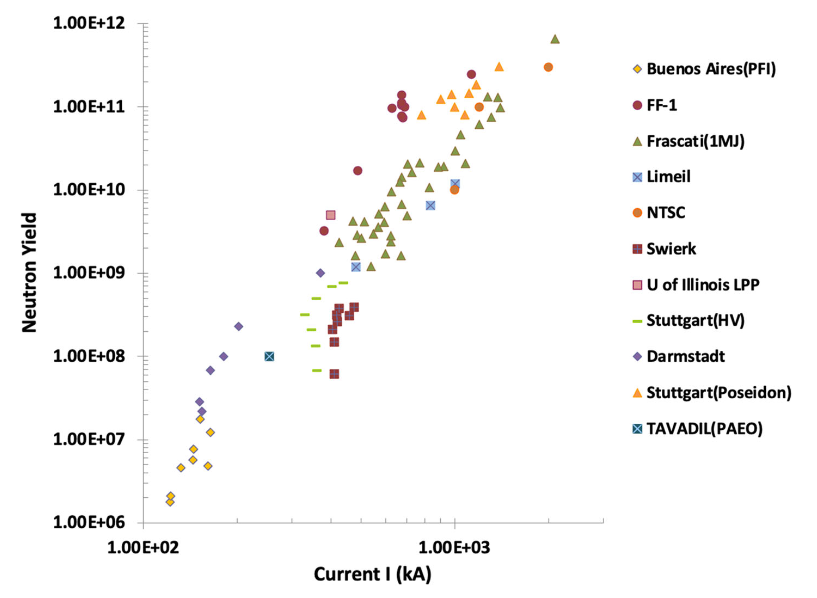
\includegraphics[width=0.45\textwidth]{figures/fusion-yield.png}
        \caption{Up to peak currents of 1MA, DPF fusion yield rises sharply with increasing current, but plateaus above 1MA. At lower currents, FF-1's performance exceeds those of other DPFs, but was comparable to other best results at 1MA. \cite{lerner_2023_focus}}
        \label{fig:fusion-yield}
    \end{figure}

    E. J. Lerner, S. M. Hassan, I. Karamitsos-Zivkovic, and R. Fritsch. Focus Fusion: Overview of Progress Towards p-B11 Fusion with the Dense Plasma Focus.
\end{frame}
\section{Theoretical Advances by LPPFusion Researchers}
\begin{frame} {Quantitative Model of DPF Functioning}
    \begin{align}
        r_c & = 1.32\times10^{-3}(\mu\cdot z)^{-2/3}r \\
        B_c & = 4z\left(\frac{\mu M}{m}\right)B       \\
        n_c & = 3.7\times10^{10}\frac{\mu^2zI^2}{r^2} \\
        Y   & \sim \mu^{2.75}I^4f(T_i)
    \end{align}
    where $B$ is peak field at cathod (G), $B_c$ is the field in the core of the plasmoid, $r$ is cathode radius (cm), $r_c$ is the plasmoid core radius, $n_c$ is plasmoid ion density, $I$ is peak current (A), $\mu$ is average ionic mass, $z$ is ionic charge, $Y$ is fusion reaction number and $f(T_i)$ is the reaction rate as a function of ion temperature $T_i$.

    Conclusions:
    \begin{itemize}
        \item $I^4$ scaling is correctly predicted by the model.
        \item Yield increases with increasing atomic mass of the fill gas.
    \end{itemize}
\end{frame}

\begin{frame} {Quantum Magnetic Field(QMF) Effect}
    \begin{itemize}
        \item Problem of high X-ray emission with p-B$^{11}$ can be mitigated through the use of quantum magnetic field (QMF) effect.
        \item In strong magnetic field, electrons can have only discrete energy levels, termed Landau levels.
              \[ E_b = \left(n + \frac{1}{2}\right)\frac{e\hbar B}{mc} \]
        \item Very little energy can be transferred from ions to electrons by collisions.
    \end{itemize}
\end{frame}

\begin{frame} {Control of Angular Momentum and Efficiency of Energy Transfer to the Plasmoid}
    \begin{itemize}
        \item For high efficiency, control of angular momentum is required.
        \item The plasmoid formation requires certain amount of angular momentum, so that kink instability can occur.
        \item Angular momentum can be imparted to the plasma sheath during the rundown by the interaction of the inward flowing electron flows and any small initial axial magnetic field. $\mathbf{J\times B}$ accelerates the electron in the azimuthal direction.
    \end{itemize}
\end{frame}

\begin{frame} {Viscous Heating Mechanism}
    \begin{itemize}
        \item Ions in the plasmoid might be heated by viscous heating.
        \item As plasmoid contracts, ions moving inward at different velocities start to mix. The ordered velocity of motion is converted into random velocity of heat.
              \[ T_i = 6.2\times 10^{-4} z_{eff}^{1.6} n_i^{0.2} (\ln\Lambda L_{max}B)^{0.4} \]
              where $z_{eff} = (\sum fz^2)^{1/2}$, $f$ is the number fraction of a given ion, $z$ is the ionic charge and the summation is over all ions. $z_{eff}$ is thus a dimensionless number, the effective number of charges per ion. $L_{max}$ is the distance around the plasmoid, which in our model is $9.7(\mu z)^{1/3}L_p$, where $L_p$ is the observed length of the plasmoid core along its axis. $T_i$ is the ion temperature in eV.
        \item Higher $T_i$ can be expected with higher $z$ fill gas.
    \end{itemize}
\end{frame}

\begin{frame} {Induced Current Heating Mechanism}
    \begin{itemize}
        \item Electron beam induces currents in the plasmoid electrons.
        \item Plasmoid has a great density, this current is distributed over these electrons.
        \item The slow electrons undergo collisions and converted their kinetic energy to heat.
              \[ T_e = 0.19(z_{eff}/r_b)^{0.8}(\ln\Lambda LI/z(\gamma-1))^{0.4} \]
              where $r_b$ is the beam radius and $\gamma$ is the relativistic factor for the beam electrons.
    \end{itemize}
\end{frame}

\begin{frame} {Lower Hybrid Heating Mechanism}
    \begin{itemize}
        \item For the densest plasmoids, lower hybrid instability will lead to wave heating of ions by the electron beam.
        \item For current more than $I>5.0/\mu^{1/6}z^{5/6}$\unit{\mega\A}, the majority of electron beam energy will go to ion heating, rather than electron heating.
    \end{itemize}
\end{frame}

\begin{frame} {Role of Impurities of Disrupting Filaments and Source of Impurities}
    \begin{itemize}
        \item High z impurities increase radiation, limiting fusion yield.
        \item High z impurities decrease the conductivity of the plasma in the current-carrying sheath, leading to disruption of the filaments through over heating.
        \item High z impurities reduces density (and hence yield) due to asymmetric compression.
        \item The increasing presence of impurities is hypothesized to be the main reason for the plateauing of fusion yield.
    \end{itemize}
\end{frame}

%%%%%%%%%%%%%%%%%%%%
% references
%%%%%%%%%%%%%%%%%%%%
\newpage
\begin{frame}[allowframebreaks]
	\bibliographystyle{abbrv}
	\bibliography{../references}
	\nocite{*}
\end{frame}

\end{document}
